\RequirePackage[hyphens]{url}

% see https://www.usenix.org/conferences/author-resources/paper-templates
\documentclass[letterpaper,twocolumn,10pt]{article}
\usepackage{usenix,epsfig,endnotes}

\usepackage{url}
\usepackage{hyperref} 
\usepackage{breakurl} 
\usepackage{graphicx}
\graphicspath{ {images/} }
\usepackage{subfigure}

\begin{document}

\date{}

% 1) Title - something that describes the nature of the project
\title{\Large \bf Exploring the Feasibility of a Scalable Internet Payment Architecture}

\author{
{\rm Ed Oakes} \\
{\rm \texttt{oakes@cs.wisc.edu}}
\and
{\rm Keith Funkhouser} \\
{\rm \texttt{wfunkhouser@cs.wisc.edu}}
}

\maketitle

% Ads
% Ad-blockers
% Auctions
% Current solutions

% 2) Abstract - provide a terse description of the problem you are addressing, why it is important and what you intend to do
\begin{abstract}
Online advertising revenue continues to climb higher each quarter.
The growth of ad-blockers has been cause for alarm for many of the primary stakeholders in this complex ecosystem.
Previous attempts have been made, unsuccessfully, to incorporate micropayments for content producers into the fabric of the internet.
Here, we investigate scalable, performant, and easy to use extensions of the internet payment architecture which address the concerns of both internet users and publishers.
\end{abstract}


% 3) Overview - similar to the abstract, provide a description of the motivation, challenges, RESEARCH QUESTION (which should be separated from the rest of the text and written in BOLD font), proposed approach (one paragraph) and expected outcomes.

\section{Overview}
Historically, online advertising has served as the primary source of revenue for content creators.
This framework has catalyzed the rapid growth of the internet, as consuming quality content for free is extremely attractive to users.
However, producing such content is not free for publishers who are currently left with two options: sell space on their site to advertisers, or move to a subscription-based model.
Advertisements have largely won this battle, partially due to a few key examples of the “paywall” architecture failing to retain users~\cite{nyt}.
This has led to a modern internet which is filled with publishers entirely reliant on the ads that keep their lights on.

Here, we explore an alternative payment system, Harpocrates, which provides users with a choice to avoid advertisements on the internet and still compensate publishers.
In designing the architecture, we focus on two key factors: convenience and scalability.
The ultimate goal is to minimize the burden on the user by providing a payment system which integrates into the current internet ecosystem, while designing an architecture flexible enough to scale with the internet.

We also describe proof of concept browser extension modifications, ``\textit{Un}acceptable Ads'', which allow users to specify the quantity and type of ads that they want to block, offering an immediate compromise between the negatives of ads for users and the need for publishers to be compensated.

Ultimately, the research question explored was: \\
\\
\textbf{Can we devise a scalable internet payment architecture that supports ad-free browsing for users and fair compensation for content publishers?}


\section{Background}
\subsection{Online Advertising}
In fiscal year 2016, internet advertising revenues in the United States totaled \$72.5 billion (a 21.8\% increase over 2015)~\cite{iabfy2016}.
Increasingly, much of this money is going to mobile advertising; in the first half of 2016, mobile surpassed search for the first time as the leading ad
format~\cite{iab2016}.
In such a massive and diverse industry, the technology surrounding the online ad ecosystem has grown exceedingly complex.
Online ads can be sourced via premium campaigns, ad networks, or ad exchanges and involve detailed targeting and accounting mechanisms~\cite{adscape}.
The number of players involved is constantly increasing, raising the barrier to disrupt the industry higher than ever ~\cite{lumascape}.

\subsection{Ad-blockers}
The growth of ad-blockers in recent years has been cause for alarm for many current online advertising stakeholders.
In a recent study of 2 million users, Malloy et al. found U.S. ad-blocker penetration to be 15.7-18.6\% (95\% CI)~\cite{malloy}.
An active measurement study by Pujol et al. estimated that 22\% of users were likely using ad-blockers~\cite{pujol}.
Surveys by various entities in the advertising industry have estimated that 26\% of desktop users~\cite{iab-blockers} and 37\% of mobile users~\cite{gwi} are blocking ads in the U.S.
Another industry survey estimates that 309 million are using mobile ad-blockers globally (16\% of global smartphone users)~\cite{pagefair}.
A simple back-of-the-envelope calculation reveals the scale of the impact this has on content providers: using the most conservative of the above ad-blocker estimates (15.7\%) and the \$72.5 billion spent in FY 2016, publishers, marketers, and others are missing out on approximately \$11.38 billion in revenue per year due to ad-blocking users.
We note that this can even be considered a conservative estimate, as a 2015 study by Adobe and PageFair estimated the cost to be \$20.3 billion in 2015, and predicted that it would grow to \$41.4 billion by 2016~\cite{pagefair2015cost}.
As both the quantity of money invested into digital advertising and number of ad-blocking users grow, this figure is becoming increasingly significant~\cite{iab2016}.

In response to this growth in ad-blocking technology, a new breed of partnerships are forming.
Eyeo GmbH, which makes Adblock Plus (installed on over 100 million active devices~\cite{abp}), began its Acceptable Ads program in 2011, which allows “large entities” to pay in order to have their ads whitelisted for its users.
As of 2015, this list was known to include Google, Microsoft, Amazon, and Taboola~\cite{whitelist}.
Increasingly, the battle over ad-blockers is being fought in the courtroom.
Recently, a German court banned Eyeo from collecting money from German publishing house Axel Springer~\cite{axel}.
These battles point to the higher-level rejection of advertisements by users, and suggest that a more sustainable compensation model is necessary for the long-term internet to continue to attract users and reward content producers.


% 4) Related work - provide descriptions of the key research papers (at least 3) related to your proposed study
\section{Related Work}

\subsection{Academic}\label{academic_related}
The idea of using ``digital cash'' to facilitate transactions online experienced substantial popularity in the late 1980's and early 1990's.
Chaum was one of the first to introduce the concept of an anonymous, untraceable micropayments (then, a ``blind signature cryptosystem'')~\cite{chaum1983blind}.
Later, this work was expanded to prevent duplication of coins~\cite{chaum1990untraceable}, and eventually spun off into the company DigiCash~\cite{schoenmakers1998security}.
Dukach's SNPP (Simple Network Payment Protocol) represents one of the first fully-described micropayment protocols~\cite{dukach1992snpp}.
Wheeler~\cite{wheeler1997transactions} and Rivest~\cite{rivest1997electronic} studied ``probabilistic'' micropayment schemes, in which the ``bank'' only cashes a small percentage of ``checks'', but in the long run everyone ends up paying the correct amount of money.
This work spawned the startup Peppercoin, which was eventually acquired.
Work at DEC on Millicent~\cite{manasse1995millicent} inspired Rivest and Shamir's work on two schemes, PayWord (credit-based) and MicroMint (less secure but faster)~\cite{rivest1997payword}, although these same ideas had been proposed shortly before by Anderson et al.~\cite{anderson1997netcard}.
IBM developed a micropayment-based extension for their \textit{i}KP macropayment system~\cite{hauser1996micro}.

Although each of these projects had unique approaches to architecture and implementation details, the design parameters primarily revolved around some subset of anonymity, reliability, trust, scalability, usability, and security. Some work has been done to classify and characterize these manifold schemes across various axes~\cite{abrazhevich2001classification,parhonyi2005second,parhonyi2006fall}. They each foresaw the advent of small transactions on the Web for content like music (e.g. \$1 songs on iTunes), however the majority of work was invested in the technology rather than supporting and increasing adoption. In particular, the need for widespread adoption of a micropayment system by both customers and sellers led to the eventual death of each system in its own time.

\subsection{Commercial}
Interest in online microtransactions has experienced a growing resurgence over the last decade.
As the use of ad-blocking software continues to grow worldwide, publishers and users alike realize that we must consider new models for financing the Web as we know it.

One such attempt is a model which participates in ad auctions on behalf of the end user, such as Google's Contributor program~\cite{contributor}, which is now discontinued, and Atri~\cite{atri}.
Though this approach will tend to find the market value for space on a given page, it includes network and computational overhead in order to participate in auctions before serving the page.
This limits the performance benefit of removing ads from internet browsing, and also requires building and installing software to participate in each ad exchange.
Additionally, Google Contributor was limited exclusively to advertisements served via Google AdSense, which resulted in a user experience which was only partially ad-free~\cite{adsense}.

Brave, a fork of the Firefox project, is a new browser which allows users to divide up a monthly subscription to the sites that they visit most often via Bitcoin-based micropayments~\cite{brave}.
The project uses the cryptographically secure Anonize protocol~\cite{anonize} to prevent a user's browsing history from being linked to their identity.
Systems like these will face scalability concerns with organizing payments when dealing with a large number of content producers and consumers.
Additionally, requiring the use of an entirely different browser adds a barrier of entry for new users.

Sourcepoint~\cite{sourcepoint} and Blendle~\cite{blendle} offer consumers a “content pass” which allows them access to a variety of content providers for a monthly subscription.
This approach is very similar to the ``paywall'' which is currently implemented on many major publisher sites, and will require cooperation from many large publishing players in order to be feasible at a larger scale.

SatoshiPay~\cite{satoshi} and Autotip~\cite{autotip} allow users to send micropayments in Bitcoin.
However, Bitcoin transaction fees have increased so much in recent years that micropayments are almost infeasible.

Flattr Plus~\cite{flattrplus} (a partnership between Flattr and Adblock Plus) allows consumers to distribute a monthly subscription among selected content provides.
Although the intersection of these two user bases is quite large (ad-blocker users and those who want to contribute to content providers), the implementation currently uses a browser extension to track user behavior, leading to privacy concerns


% 5) Methods - provide a description of the way in which you intend to address the research question.  This means describing the existing tools/systems that you will use, new tools or systems that you will build and the experiments that you will conduct.
\section{Harpocrates}
In this section, we present our design for a system, Harpocrates (Greek god of silence, secrets, and confidentiality), which allows users to easily compensate publishers at a fair rate for their content without being forced to view ads.
Harpocrates is composed of a client-side browser extension for users to configure their preferences and a server for bidding on ad placements and accounting of payments between users and publishers.
The main focus of Harpocrates is that it fits into the current ad ecosystem with minimal implementation work required for publishers.

\subsection{Design Considerations}
In designing Harpocrates, there was a clear set of requirements which, if not accomplished, would yield a system infeasible for wide deployment.

First, the system must address the concerns of current ad-blocker users. This is the number one design principle, as if the system doesn't provide users with at least a subset of the benefits they receive from blocking ads, they won't even consider using it. We define these concerns as three main considerations: intrusiveness, performance, and security/privacy, derived from a 2016 HubSpot survey of 731 Adblock Plus users on why they block ads~\cite{hubspot2016adblock}.

The system must also be as unobtrusive to the user as possible.
Web users are accustomed to convenience and an uninhibited browsing experience, and our system should follow this pattern to attract users.
For example, with our current design, there is a very simple settings page which a user need only visit once at minimum, allowing them to specify their budget.
Beyond that everything is handled on the back-end.

The system should fit into the current Web ecosystem.
This means that we cannot rely on any new standards or widely-implemented protocols in order to see wide adoption.
Correspondingly, the implementation cost for publishers must be minimized, because it will never see wide adoption if it requires a complex or custom implementation for each publisher.
This excludes solutions that involve adding significant server-side code, such as nearly all of the services described in Section ~\ref{academic_related}.
Another key piece to fitting into the Web payment infrastructure is that our system needs to be able to coexist with ad networks as they exist today.
Many Web publishers survive exclusively off of ad revenue, and they cannot be expected to switch to an entirely new compensation model which abandons the tried-and-true ad revenue model.

Finally, the system must provide control over the browsing experience for both users and publishers alike.
Currently, publishers are essentially locked in to using a combination of subscription and ad tactics for revenue and users are locked in to paying for these subscriptions and seeing ads across the Web.
We want to provide an alternative which can be opted into and out of easily for both publishers and users, which lets them shape their own browsing experience.
By enabling publishers to recoup some of the lost revenue due to blockers, and enabling users to opt-in to funding their favorite content, both parties benefit.

\subsection{Architecture}
Ultimately, Harpocrates can be seen as a Web ad network, which places ``blank ads'' instead of images or videos and whose advertisers (those paying for the ad placements) are the users themselves.
Users specify a monthly ``budget,'' which Harpocrates then uses to bid on each ad that a publisher wants to sell.
This design very cleanly fits into the current ecosystem, and requires very minimal effort from the user: they only have to register with one entity, Harpocrates, and they need only set their preferences at least once in order to get off the ground, directly compensating publishers and seeing fewer ads.
This solution relies on fact that publishers ad servers and ad exchanges are efficient marketplaces for determining the fair value for a given piece of ``real estate'' on the internet.
In order to take advantage of this fact, Harpocrates sits inline in the ad ``waterfall'' that currently exists in many publisher ad servers (Figure ~\ref{fig:waterfall}).

\begin{figure}[t]
\centering
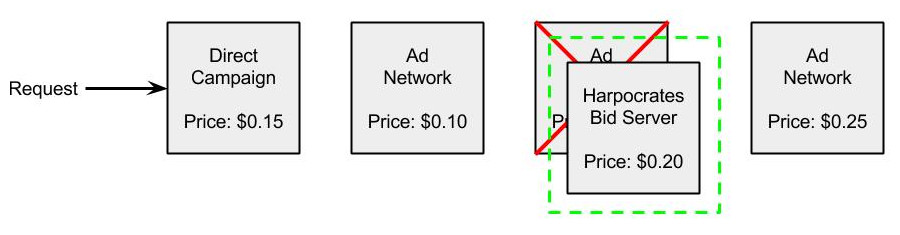
\includegraphics[width=0.5\textwidth]{waterfall}
\caption{Harpocrates sits inline with the current ad exchange ecosystem.}
\label{fig:waterfall}
\end{figure}

From the publisher's point of view, Harpocrates is essentially no more than another ad network, which, given an impression, returns a bid for the ad (or none) based on the user's budget and the estimated value of the ad space.
This allows the publisher to choose whether or not to use Harpocrates at a per-ad granularity, and its implementation cost is no higher than that of adding another ad network, requiring no additional infrastructure or protocol that isn't already there.
The only piece of information which needs to be shared between publisher and Harpocrates is a user ID which associates the user who requested the page and their Harpocrates account, but this can be passed as one of the cookies which are already passed around to identify Web users.

From the user's point of view, Harpocrates is simply a browser extension  (Figure ~\ref{fig:harpocrates_ui}) which they pay some chosen amount of money to each month, and it in turn removes some of the ads that they see on their favorite sites.
They don't need to have any knowledge of the complex ad ecosystem, only that they are directly compensating the content publishers.
In addition, users can elect to fall back on blocking ads even when the Harpocrates bid server does not win a given auction.

\begin{figure}[t]
\centering
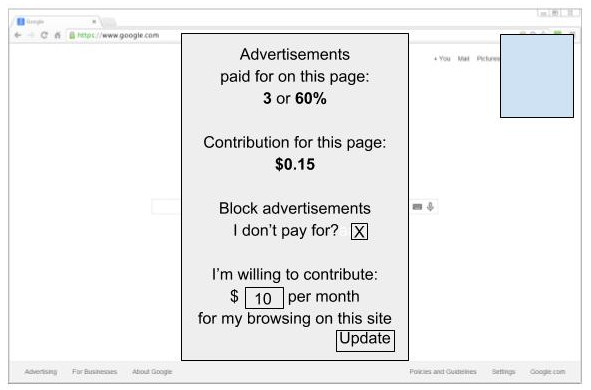
\includegraphics[width=0.5\textwidth]{harpocrates_ui}
\caption{For the user, Harpocrates simply requires installing a browser extension and initializing a few settings.}
\label{fig:harpocrates_ui}
\end{figure}

Finally, Harpocrates also acts as a clearinghouse, settling accounts monthly.
For a given set of publishers $N$ and users $M$, only $O(|N| + |M|)$ payments need to be transacted (i.e. one payment from each user to Harpocrates, and one payment from Harpocrates to each publisher).
At scale, we gain a lot from this aggregation of payments when compared to a system such as paywalls, which requires $O(|N| \cdot |M|)$ payments (one for each user/publisher pair) in the worst case.

These aspects of the architecture make Harpocrates a good candidate solution, given the aforementioned design considerations.
It addresses the needs of current ad-blocker users by showing them fewer ads, the user interface makes it practically invisible from a user's point of view, and performance is improved by eliminating the actual delivery of ad media content (Figure ~\ref{fig:harpocrates}).
Harpocrates also fits into the current complex ecosystem, requiring no new standards or protocols.
Finally, the implementation is simply adding another ad network, minimizing implementation costs.
The one design point which we do not hit is that of user security/privacy concerns.
Unfortunately, because Harpocrates doesn't restrict publishers from serving ads, and needs to be able to make market-rate bids on ad space in order to serve its purpose, user tracking is still necessary.
Despite this, however, we believe that Harpocrates' scalability and ease of use for both users and publishers makes it a promising alternative to the ad-based payment model of the internet as we know it today.

\begin{figure}[t]
\centering
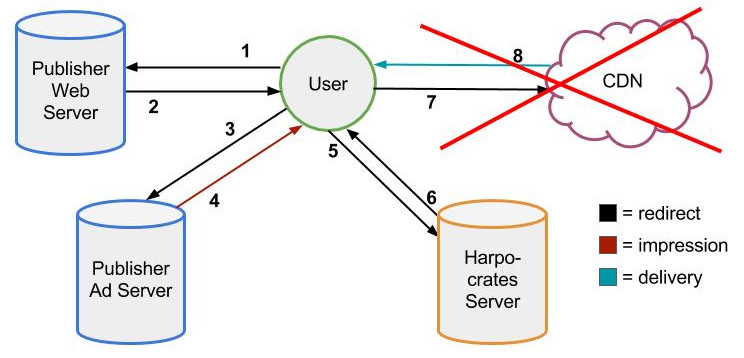
\includegraphics[width=0.5\textwidth]{harpocrates}
\caption{Harpocrates removes the actual ad media element delivery process, cutting out a roundtrip request to the ad server content delivery network and improving performance.}
\label{fig:harpocrates}
\end{figure}

\section{\textit{Un}acceptable Ads}
\textit{Un}acceptable Ads is a proof of concept to illustrate a more immediate path forwards for users who block ads because of the reduced performance and/or visual obtrusiveness.
Relying on the idea that users are willing to see some ads in order to support content publishers, our goal is to allow users to specify the number and type of ads that they do not want to see.
This idea is similar in motivation to the Acceptable Ads program run by Adblock Plus, but where Acceptable Ads are determined by the Adblock Plus organization and advertisers can pay to be whitelisted, our system will put the control directly in the user's hands.
To realize this idea, we have modified two Chrome extensions: uBlock Origin, a request-based blocker, and a ``perceptual blocker'' which was recently developed by Storey, et al.~\cite{storey2016future} at Princeton University.

\subsection{uBlock Origin}
uBlock Origin is a popular open source desktop ad-blocker with nearly 9 million installs on Google Chrome as of May 2017.
This blocker is categorized as a request-based blocker, meaning that it recognizes Web requests which are targeted at ad-related servers and prevents them from ever leaving the client's browser.
This strategy offers significant performance benefits, as it reduces network traffic and prevents (often large) media elements from being received and rendered in the client browser.
Identifying ad-related network requests is done by matching target URLs against a list of known advertising URLs (e.g., EasyList~\cite{easylist}).
The extension uses multiple such community-maintained lists, and matches against them using a combination of simple lookups and regular expressions.

\begin{figure}[t]
\centering
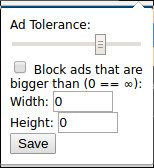
\includegraphics[width=0.15\textwidth]{unacceptable_ui}
\caption{User interface for our modification of the perceptual blocker.}
\label{fig:unacceptable_ui}
\end{figure}

Our modification to the uBlock Origin is a notion of ``Ad Tolerance'', a configurable setting from 0-100\% which determines what proportion of ads will be shown to the user on any given page.
If the user has their tolerance set to 0\%, the extension will block all ads like uBlock Origin usually does and if the user has their tolerance set to 100\% then the extension won't function as an ad-blocker at all.
Any setting between 0 and 100\% will result in each ad element probabilistically being blocked (Figure ~\ref{fig:unacceptable}).
The reason for probabilistic blocking is that it is a very difficult problem to predict the number of total ads that will be shown on a page before the page has fully rendered, so blocking a pre-determined number of elements is impractical.
While probabilistic dropping means that the proportion of ads blocked might not be exactly as expected on every page, in the long run the number of ads blocked will very closely match the specified proportion.

\subsection{Perceptual Blocker}
Storey, et al.~\cite{storey2016future} recently published work on what they dubbed a ``perceptual blocker'', which blocks ads based on their visual content rather than their associated Web requests or the structure of the page.
The primary observation which this work is based on is that there have been many efforts recently to standardize ad policies on the internet through joint coalitions such as AdChoices~\cite{adchoices}.
Such programs require ads to identify themselves by including text such as "from our advertisers" or by displaying a common logo, such as the AdChoices logo.
Storey, et al. recognized that this offers an opportunity to visually recognize and identify ads as a human would be able to.
The blocker that they developed puts this idea into practice, and covers all visually recognized ads with a banner reading "THIS IS AN AD."
Covering ads rather than completely hiding them is deliberate, as the researchers wanted to avoid potential backlash from the advertising community, which is discomforted by the idea that their ads could be completely delivered but still not presented to a user - leaving them paying for an impression which didn't actually happen.
This raises a broader question about the morality of perceptual blockers, and suggests that if these blockers were to become popular, advertisers would have to make a significant engineering effort to maintain accurate impression accounting in their presence.

\begin{figure}[t]
\hfill
\subfigure{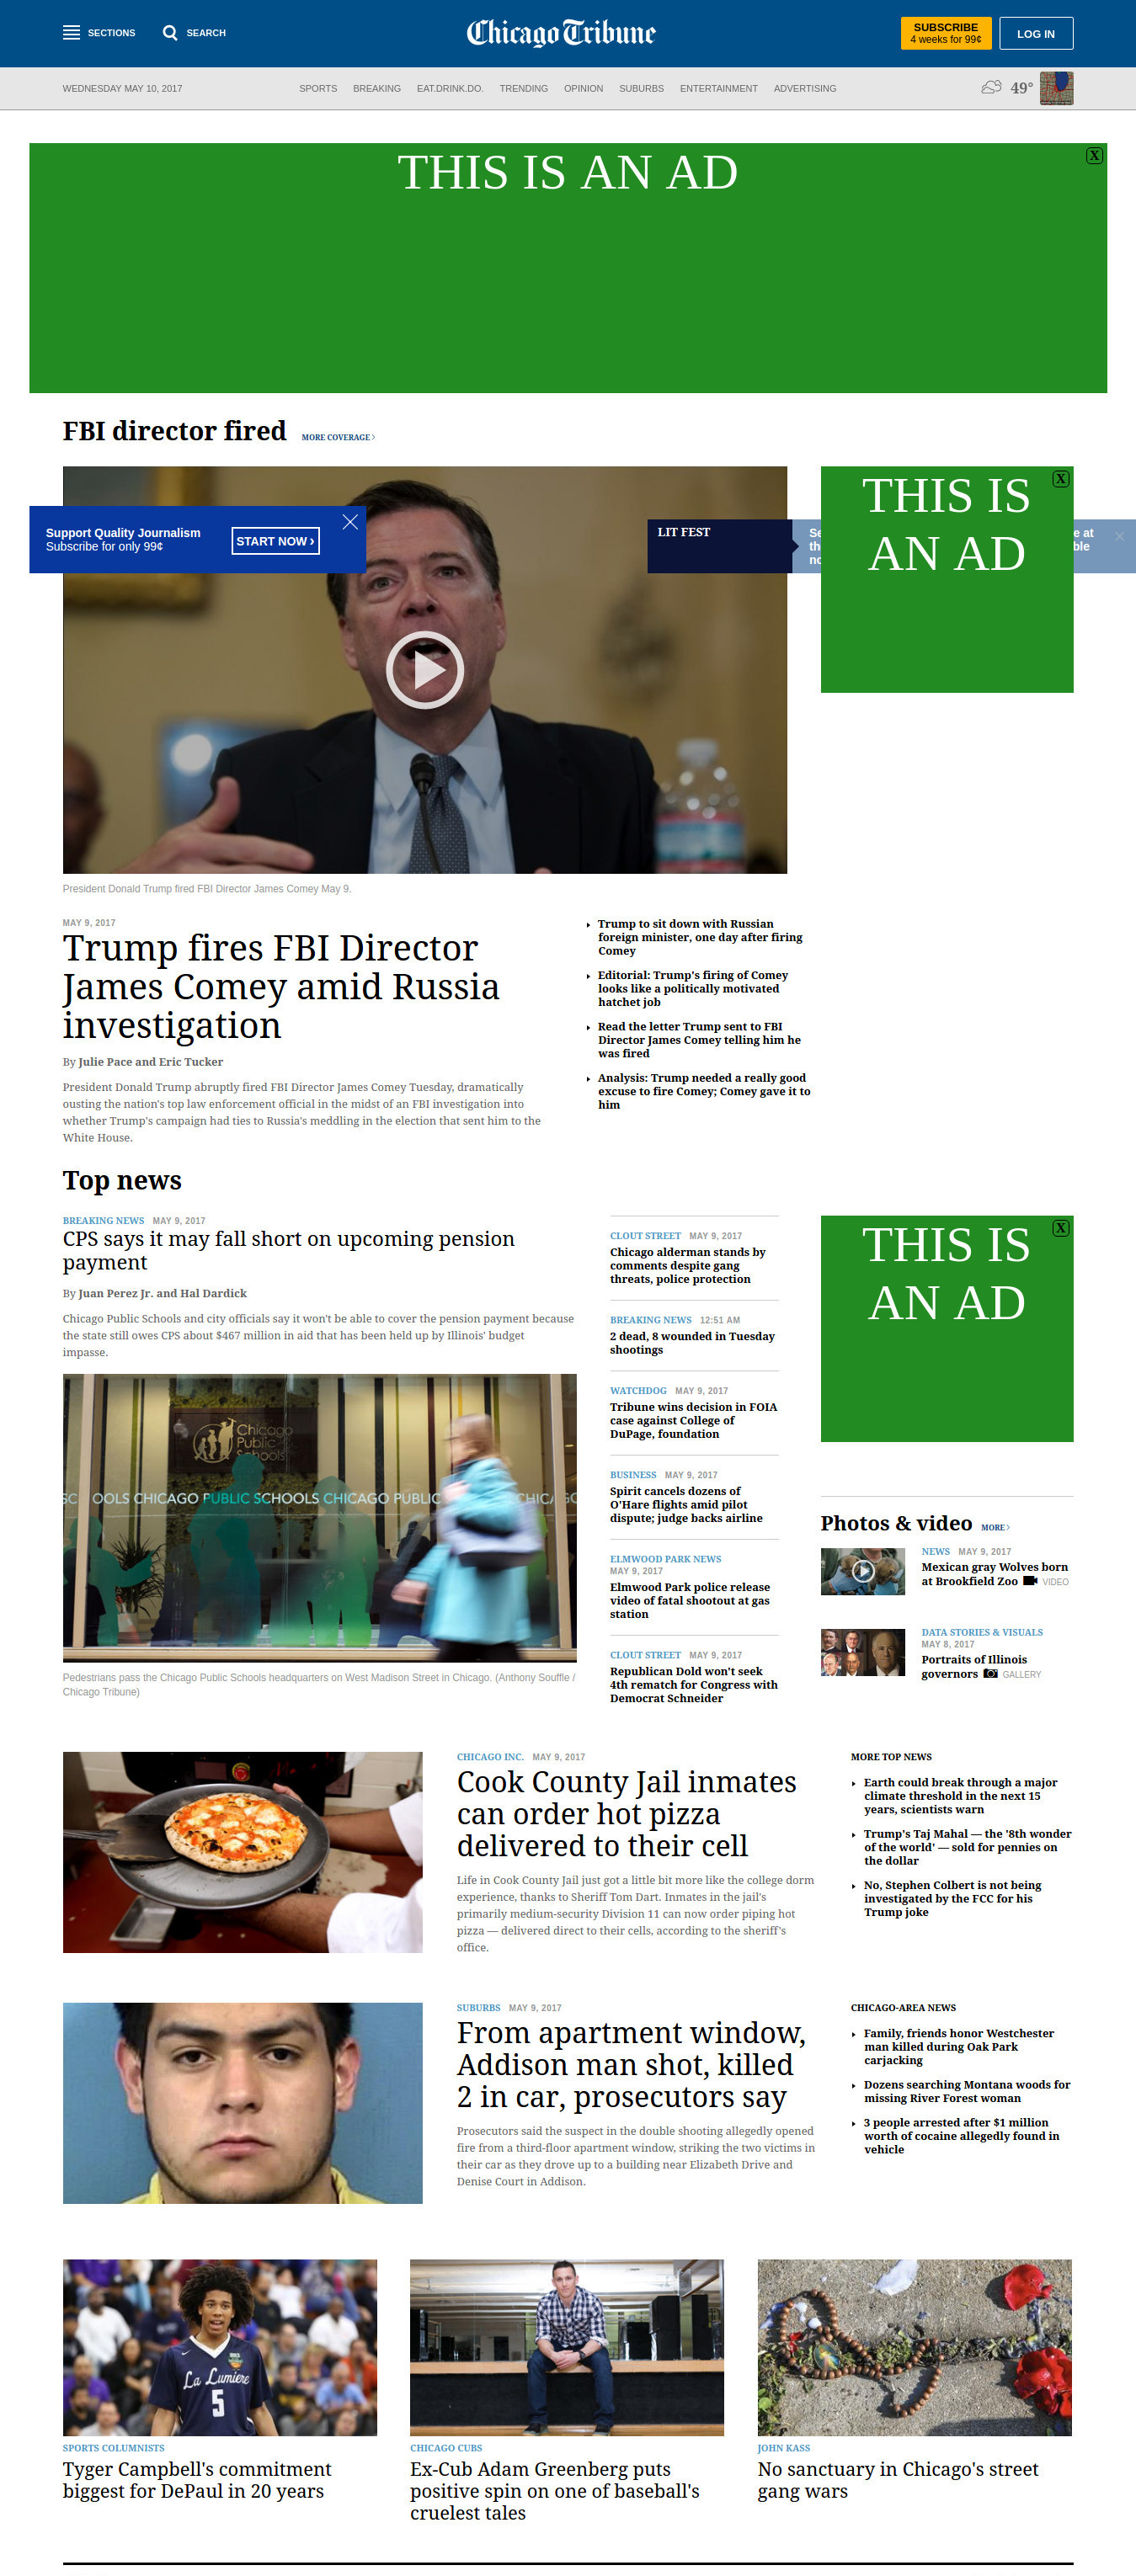
\includegraphics[width=0.15\textwidth]{unacceptable_no_tolerance}}
\hfill
\subfigure{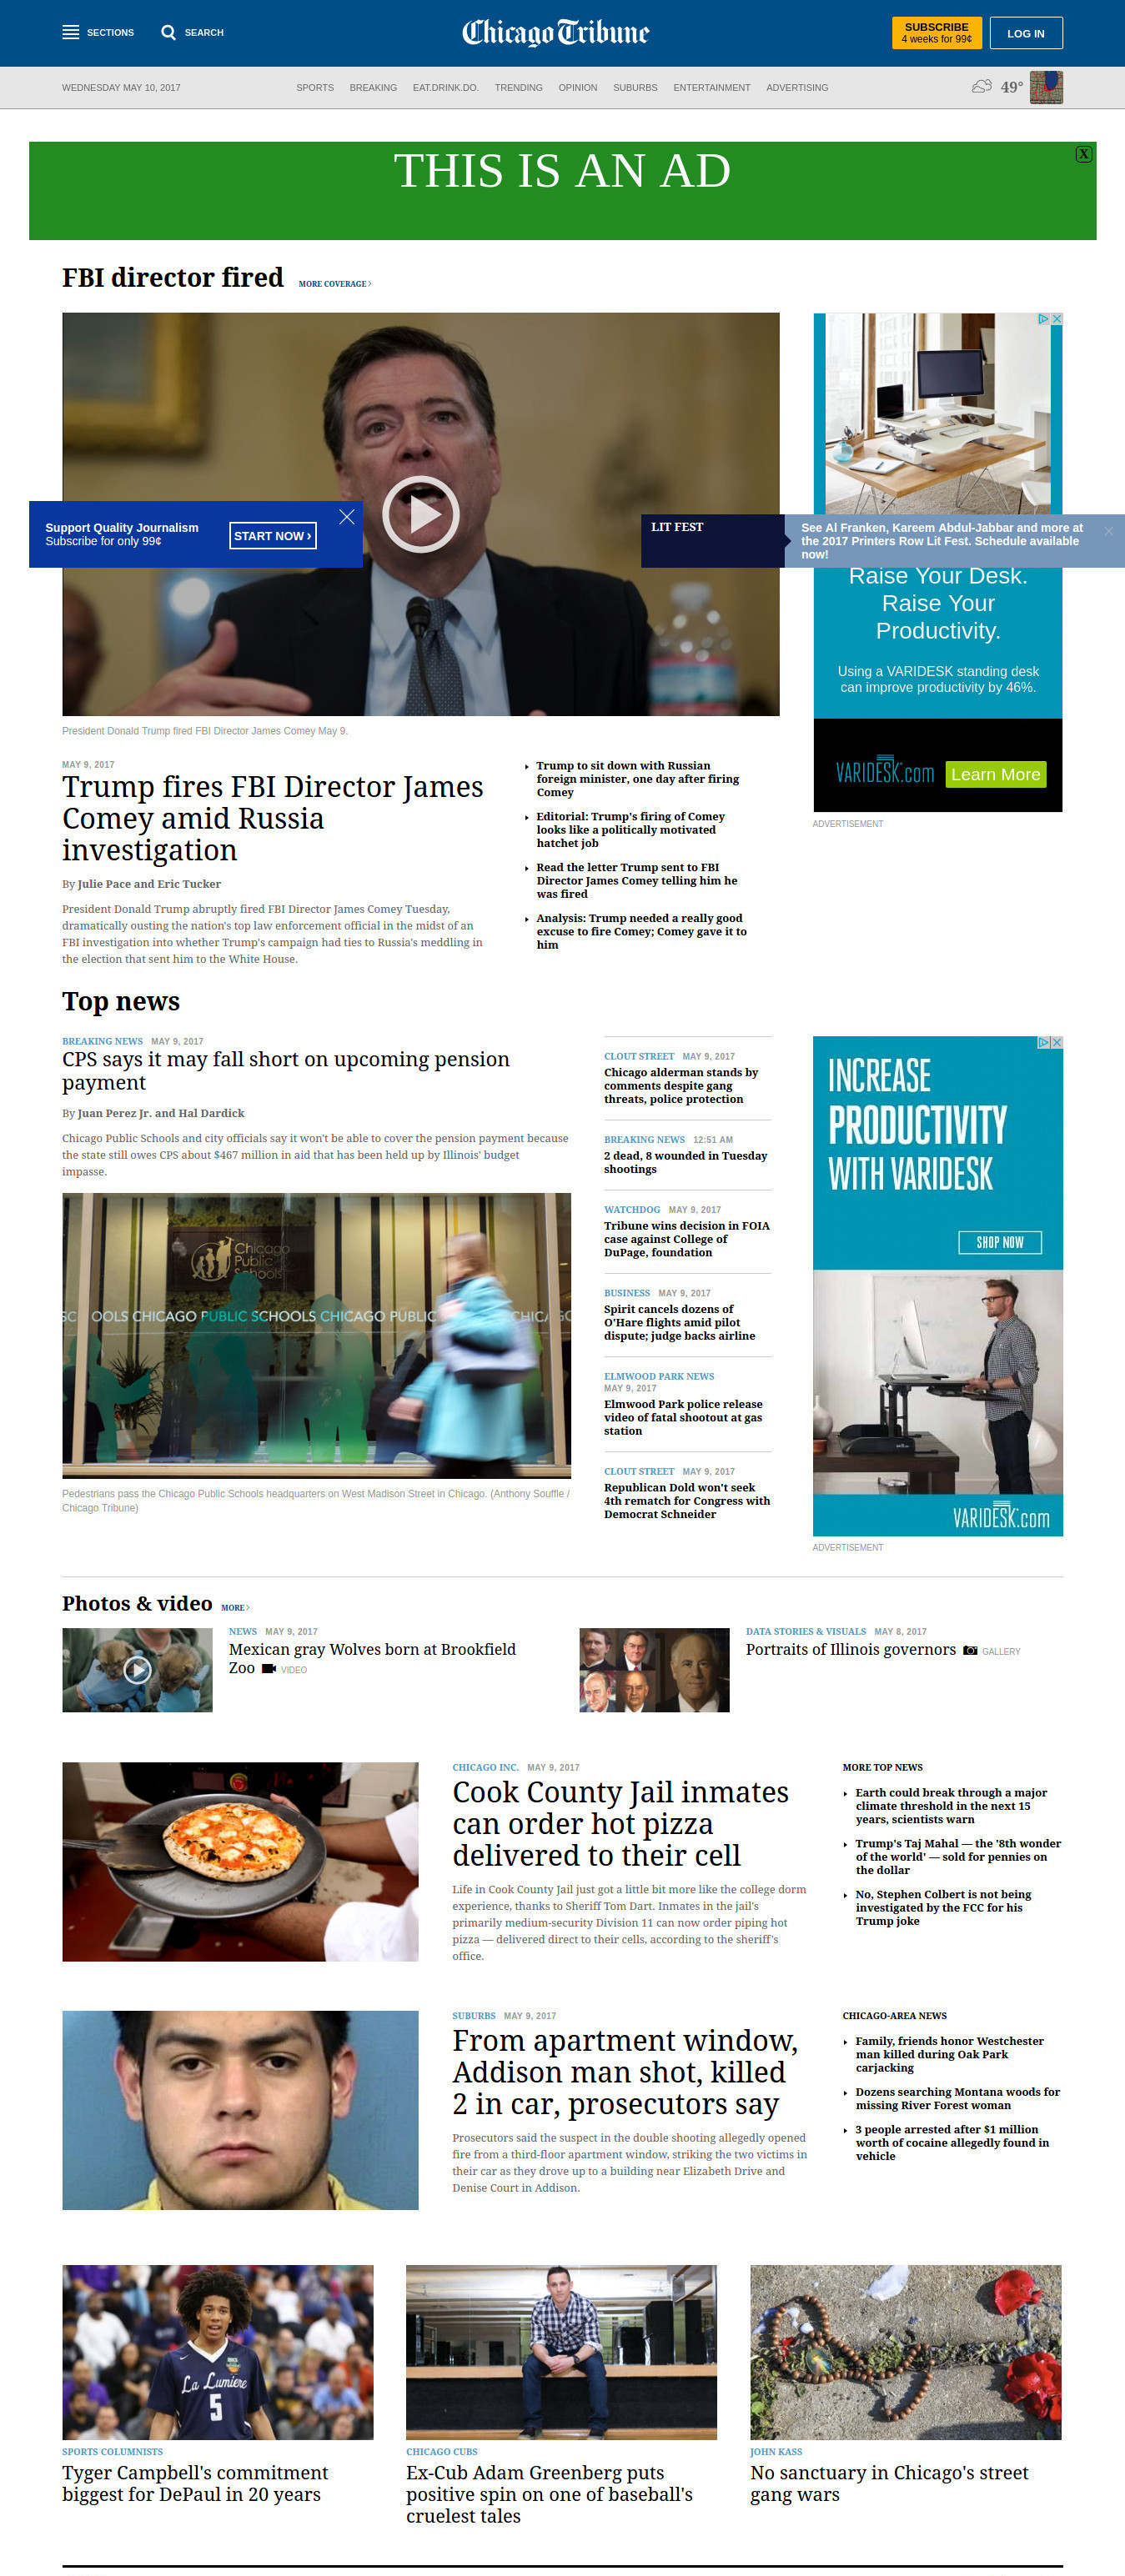
\includegraphics[width=0.15\textwidth]{unacceptable_high_tolerance}}
\hfill
\caption{\textit{Un}acceptable Ads allows the user to select their tolerance for advertisements, from 0\% (left) upwards (right).}
\label{fig:unacceptable}
\end{figure}

Our first modification to the perceptual blocker is the same as that which we made to uBlock Origin, adding a configurable tolerance level which probabilistically blocks the ads it encounters.
We also added a second configuration to this blocker, which allows the user to specify a maximum width and height of ad elements which they are willing to see (Figure ~\ref{fig:unacceptable_ui}).
This highlights a key benefit to the perceptual blocker, because the ads are completely delivered before blocking occurs, the blocker has a more complete set of information about the ad's qualities (e.g., size, content, placement on the page) when the blocking decision is made.
We use this additional information to block ads above a certain size, but this could be extended to other configurations, such as recognizing and blocking inappropriate ads.

\subsection{Performance}
In order to assess the impact of ad-blockers on performance, we performed an experiment to measure page load times with and without uBlock Origin enabled.
The five sites which we chose to measure load times on were the five most popular news sites based on the Alexa ranking~\cite{alexa}.
We loaded each site 10 times under each condition and averaged the results, closing the browser between loads to ensure that a full rendering occurred.
Page load times were measured using the Chrome extension ``Page Load Time''~\cite{pageloadtime}, which considers a page fully loaded once all elements have finished rendering.
We deliberately chose not to clear the local browser cache between page loads, recognizing that in practice Web content is often cached locally.
The results validate survey findings that many users use ad-blockers for performance reasons~\cite{hubspot2016adblock}, as there was an average of a 2.33x speedup in load time with uBlock Origin enabled (Figure ~\ref{fig:load_times}).

\begin{figure}[t]
\centering
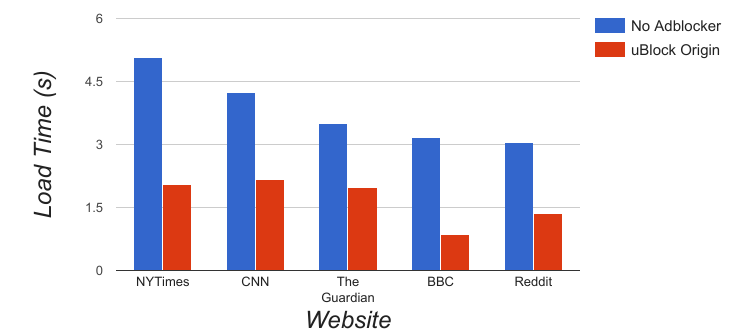
\includegraphics[width=0.5\textwidth]{load_times}
\caption{Loading times for five popular Websites with and without the popular ad-blocker uBlock Origin.}
\label{fig:load_times}
\end{figure}

To assess the performance of our \textit{Un}acceptable Ads extensions, we performed a similar experiment by measuring page load times for the Chicago Tribune homepage at multiple different levels of ad tolerance.
Our findings are consistent with our intuition: since uBlock Origin blocks based on network requests, performance should decrease as tolerance goes up.
For the perceptual plocker, however, performance stays relatively constant regardless of tolerance, since ads are detected and hidden after they are loaded (Figure ~\ref{fig:load_times_over_range}).
This difference highlights the key benefit to request-based blockers: performance.
Preventing Web requests from ever leaving the client browser results in a decrease in network traffic and the costly rendering of media elements.
One thing to note is that we consider a page to be done loading when the page is fully rendered, but this doesn't include the additional time required in the case of the perceptual blocker to identify and cover ads.
While this occurs quickly, there is some computational overhead associated with visually scanning the Web page which should be considered when comparing the two techniques.

\begin{figure}[t]
\centering
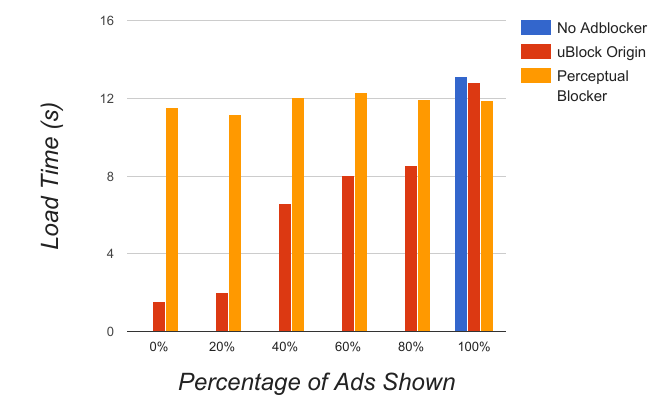
\includegraphics[width=0.5\textwidth]{load_times_over_range}
\caption{Loading times for Chicago Tribune homepage with varying levels of tolerance for ads using the \textit{Un}acceptable Ads extensions.}
\label{fig:load_times_over_range}
\end{figure}

\subsection{Summary and Technical Challenges}
These extensions serve as two separate proofs of concept for a new generation of ad-blockers which could allow for a more fine-grained tuning of what types of ads are blocked.
This approach can provide partial or full compensation for the publisher while still addressing user concerns about the performance and/or visual issues associated with ads.
We note that this solution does \textit{not} address the needs of users whose foremost concern is privacy, and leave that concern for future work.

There was a large difference in the technical challenge presented by making modifications to uBlock Origin compare to the perceptual blocker.
In the case of the perceptual blocker, the ad recognition and covering sections of the code were completely separate, allowing us to add our tweaks to the covering code (only called when an ad is recognized) in only a few simple lines.
Our understanding of the extension was also aided by the fact that the perceptual blocker was well-commented and is more of a proof of concept than a production-ready piece of software, meaning that there were far fewer optimizations and less corner-case handling.
This simplicity allowed us to easily fit our modifications in to only one section of the code with minimal debugging pain.
On the other hand, uBlock Origin is a more complicated piece of software and includes many optimizations to reduce the memory footprint and computational overhead of its ad-blocking.
Additionally, although the extension is open source, it is almost entirely maintained by a single developer.
While there is a fairly complete wiki explaining the design of the extension, the code itself is quite barren of comments.
This led to many hours spent just trying to figure out the end-to-end workflow of blocking a single ad, which involves 3 different identification mechanisms (dynamic URL filtering, dynamic host filtering, and static URL filtering) as well as a caching mechanism to prevent redundant lookups.
Our first iteration simply probabilistically let through ads which had been marked by one of the identification mechanisms, but this turned out to block far too many ads.
The excessive blocking occurred because a given ad may have upwards of 10 redirects and requests associated with it, and blocking any of these would prevent the ad from being served.
This led us to come up with a better solution: adding a second, position-based, cache which identified the position on the page of the iframe associated with an ad-related request and made a single decision to block or allow all requests for that iframe.
Although not perfect (multiple ads could have the same position, positions could change, etc.), this additional cache provided far more predictable and accurate results.
This development time was definitely well-spent, as we learned not only how ad-blockers function in practice, but had the opportunity to learn some Javascript and the anatomy of browser extensions, both of which are integral parts of the modern Web and aren't something we've worked with in the past.

Looking forward, there are many more directions to explore with this idea of user-configurable ad-blocking.
For example, while a request-based blocker doesn't allow for blocking based on a display size threshold, one similar option that could be implemented is blocking based on media element size (i.e., in bytes).
The size of an element is often included in the metadata of a redirect from an advertiser server, so blocking based on a simple check could be implemented trivially.
One issue with this approach, however, is that we must still go through the chain of redirects which determine what ad will be served and log the impression on the publisher's end.
Blocking an ad after these requests have occurred puts some stress on the publisher and marketer servers, and reduce some of the performance benefit realized on the user end.
Additionally, a blocker could block specific types of ad media elements which the user deems too intrusive (e.g., video advertisements or images that make up the background of the page).

\subsection{Code Repository}
We have made our code for the \textit{Un}acceptable Ads extensions available here:

\url{https://github.com/edoakes/740adblocker}


{\footnotesize \bibliographystyle{acm}
% 6) Bibliography - list related work using standard bibliographic form.  Simply listing titles and providing web links is not acceptable.
\bibliography{biblio}}

%\theendnotes

\end{document}
